%Project Narrative
\documentclass[12pt]{article}
\usepackage[margin=1.3in]{geometry}
\usepackage{color}
\usepackage{graphicx}
\usepackage{url}
\usepackage{multicol}
\usepackage{wrapfig}
\usepackage{amsmath}
\usepackage{amssymb}
\usepackage{caption}
\usepackage{subcaption}
\usepackage[round]{natbib}
\bibliographystyle{abbrvnat}
\setcitestyle{authoryear,open={(},close={)}}
\usepackage[usenames,dvipsnames,svgnames,table]{xcolor}
\usepackage[innercaption]{sidecap} % side captions
\sidecaptionvpos{figure}{c}

\newcommand{\jri}[1]{\textcolor{blue}{ \emph{\scriptsize  #1}} }
\newcommand{\kc}[1]{\textcolor{violet}{ \emph{\scriptsize  #1}} }
\newcommand{\citex}{\textcolor{red}{\textbf{(CITE)}}}

\begin{document}

\title{\vspace{-5ex}The genetic archaeology of maize: reconstructing pedigrees to identify useful diversity for breeding\vspace{-4ex}}
\author{}
\date{}
\maketitle

\section*{Rationale and Significance}
\label{sec:rationale}

Maize is a natural resource of fundamental national importance, vital for food, livestock feed, and fuel production.
Maize is also the most valuable field crop in the United States, with production values at greater than \$50 billion dollars every year since 2010 \citep{Tho98w}. 

But while maize yields have increased over the last several decades, the rate of gain falls short of projected needs in the near future \citep{grassini2013distinguishing}.
Even under stable climatic conditions, current rates of maize improvement are insufficient to meet requirements of population growth over the next 30 years \citep{ray2013yield}; in  addition to requirements in terms of food and animal feed, worldwide ethanol use is projected to increase 40\% within just the next decade \citep{wtf2015usda}.

Changing climatic conditions, however, will likely further challenge our ability to meet needed yield gains. 
Historical analyses suggests that climate change over the last 30 years has already dramatically impacted maize yields worldwide, retarding gains from breeding and management \citep{Lobell2011}.
Moreover, predicted temperature increases will increase volatility in yield across the U.S. and may even decrease future yields \citep{urban2012projected}, with some models suggesting a change of even 1$^{\circ}$C could negatively impact yields by as much as 17\% \citep{lobell2003climate}; more dire warnings suggest that U.S. maize yields could drop 30-46\% below current levels by the end of the century \citep{schlenker2009nonlinear}.
It is also predicted that these climate changes will interact with and change soil properties resulting in increased fertilizer inputs \citep{rosenzweig2014assessing}, and even further interact with pests and diseases \citep{anderson2004emerging}. 
These different factors may give rise to completely novel environments far different from the ones that farmers and breeders had to contend with in the past. 
Substantial efforts will clearly be needed to preserve U.S. maize production and increase or maintain yields.  

Much of the historical gains in maize yield can be directly attributed to breeding efforts \citep{Duvick1992, duvick2005genetic}, and \textbf{ breeding must remain of central importance in order to meet increased yield demands}.  
Breeding is also of key importance in adapting maize to the challenges of changing climates \citep{Troyer2004a}, with recent models suggesting that efficient use of extant adaptive diversity in maize could significantly ameliorate the effects of climate change \citep{butler2013adaptation}.   

\subsection*{Diversity loss threatens breeding gains}

Breeding, and adaptation in general, relies critically on the availability of genetic diversity. 
This is best represented mathematically by JL Lush's famous ``breeder's equation'':

\begin{align}
R=\frac{V_A}{V_P}s
\label{eq:lush}
\end{align}

showing that adaptation --- the response to selection $R$ --- depends not only on the strength of selection $s$ but also directly on the amount of heritable genetic variation $V_A$ for the trait of interest \citep{kelly2011breeder}. 
The advent of modern hybrid maize breeding, the development of distinct breeding pools and the winnowing of inbreds from individual breeding programs has led to a marked decrease in genetic diversity. 
Analyzing genotypes of more than 4000 public and recently released private lines, we recently showed that the diversity available to maize breeders in current germplasm is less than half what it was in before 1950 (Figure \ref{fig:diversity}). 
With decreasing diversity available for breeding decreasing yield gains are a mathematical certainty. 

\begin{SCfigure}
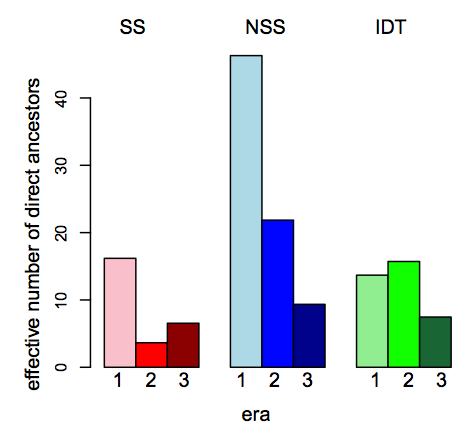
\includegraphics[width=0.45\linewidth]{joost_diversity.png}
\caption{Changes in genetic diversity (represented as the effective number of ancestors) of the three primary maize heterotic groups (SS: stiff-stalk; NSS: non-stiff-stalk; IDT: iodent). Inbreds are divided into eras representing different time periods: 1:1930-1950; 2:1950-1980; 3:1985-1992. Figure from \citet{van2012historical}.} 
\label{fig:diversity}
\end{SCfigure}

While open-pollinated varieties and exotic inbred lines represent a viable source of new diversity, these have been only sparingly used in the private sector due to their poor agronomic performance, photoperiod sensitivity, and the necessary generations of back-crossing to adapted lines required to incorporate useful alleles into high-performing temperate germplasm \citep{goodman1999broadening}.


In contrast, older U.S. inbred lines, though lower-yielding than their contemporaries, harbor novel genetic diversity of potential use for breeding \citep[e.g.][]{chen2012characterization,wisser2011multivariate}, and are already adapted to the temperate U.S.  
Breeders have clearly been successful in advancing high-yielding germplasm and discarding ill-adapted material.
This does not mean, however, that all discarded material has little genetic merit --- beneficial alleles can be lost to genetic drift, particularly considering the polygenicity of agronomic traits and also because breeders are unable to select for all traits simultaneously. Our own population genetic analysis supports this notion; a number of underutilized older inbreds are enriched with favorable alleles (Figure \ref{fig:wf9}).  

\begin{SCfigure}
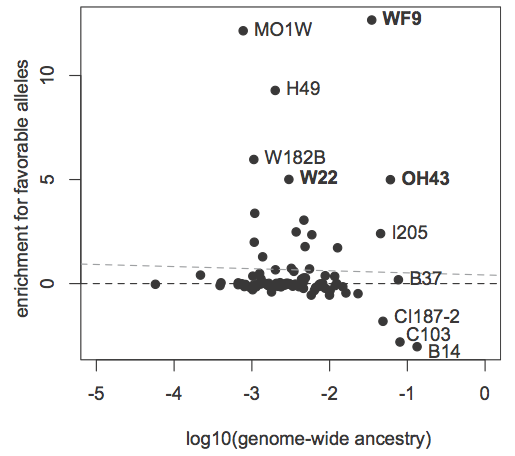
\includegraphics[width=0.55\linewidth]{joost_wf9.png}
\caption{Enrichment (log probability ratio with respect to control loci) of favorable alleles in older (era 1) inbreds as a function of average ancestral contribution to modern (era 3) lines. The gray dotted line is a  regression with slope $-0.1$). Inbred names are shown for lines with ratios higher than 4 or ancestry proportion above 0.03. Labels in boldface mark breeding lines of known historic popularity. Figure from \citet{van2012historical}.} 
\label{fig:wf9}
\end{SCfigure}

\subsection*{Lack of public resources limits use of diverse germplasm}

Breeders will not blindly incorporate older material into their populations, however.  
Perhaps the most important piece of information required to effectively utilize older germplasm is pedigree.
Pedigree data immediately gives a breeder information on crosses likely to produce higher yields due to heterosis, and often provides additional utility in identifying likely maturity (flowering time) and other agronomic characteristics. 
Combined with phenotype data, pedigrees can even be used to predict phenotype in the absence of genotype \citep{piepho2008blup} and pedigree-based methods for identifying useful diversity have already been patented by industry \citep{sebastian1995method}.

While private industry may in many cases have detailed records of their own breeding material, the vast majority of private germplasm is founded on $20^{th}$ century public breeding lines \citep{nelson2008molecular}.

Unfortunately, pedigree data for most U.S. maize inbreds is unavailable to most breeders. 
For example, of the over 45,000 worldwide inbreds in the USDA Germplasm Resources Information Network, only some 34,000 have some amount of ancestry determined, and much of this information is incomplete.
If we look at available germplasm only, that number shrinks to 2931 accessions with any available ancestry information.
While there are published compilations of germplasm, these are far from complete:  \citet{gerdes1993compilation}, for example, contains complete pedigree data for less than 20\% of the germplasm in the USDA database.
Moreover, what ancestry information that is available is not in electronic form nor easily accessible in any single resource.  
Instead, historical pedigree information exists primarily in the minutes of breeding committees, old breeding program books, and other hard-copy sources with limited distribution.  

\textbf{We propose the generation an open-source database of public maize pedigrees and use this resource to identify genotypic and phenotypic diversity of high utility in advancing maize breeding.}
Given the importance of maize to U.S. agriculture, this proposal clearly aligns with the USDA AFRI program priorities of ``Plant Breeding for Agricultural Production,'' particularly the ``development and application of tools to predict phenotype from genotype to accelerate breeding of finished varieties''.   
Our proposal will develop tools to accelerate breeding by allowing breeders to more quickly identify useful inbreds, and our application of population and quantitative genetic methods will identify specific genetic and phenotypic diversity of potential use for future breeding.  

\section*{Introduction}
\label{sec:introduction}

\subsection*{Maize breeding}
Maize has undergone dramatic phenotypic and genetic changes since its domestication and subsequent spread across the Americas \citep{daFonseca:2015ey,Doebley:2004ce}. More recently, beginning in the mid-20$^{th}$ century, the intensification of maize breeding efforts has lead to subtler but equally important changes including increasing yields and improved agronomic traits such as leaf angle and density tolerance \citep{duvick2005contribution}. 

Modern breeding programs (post-1960) take advantage of self-fertilization (or now double-haploid technology) to create homozygous inbred lines, which are maintained in separate breeding pools or heterotic groups.
The most important heterotic groups among U.S. public germplasm are the ``stiff stalk'', ``non-stiff stalk'', and ``iodent'' (Figure \ref{fig:diversity}).
Inbred lines from separate breeding pools are then crossed to make hybrid progeny.  
These hybrids often display heterosis, meaning that yield and associated traits of the hybrid are superior to  either inbred parent \citep{Springer:2007bj}.  
Inbreds capable of producing high-yielding, heterotic offspring are said to have good ``combining ability'', and are recycled in their respective breeding pools.
Inbreds that form less desirable hybrid combinations are usually discarded from the breeding pool. 
Useful inbreds within a group are crossed with each other, and their segregating progeny evaluated and self-fertilized to create new inbreds. 
Maintaining this system for propagation of inbred lines and hybridizing inbreds for evaluating production traits has worked well for many decades, but there is growing reason for concern that this method may need a genetic boost. 

\subsection*{Decelerating yield gains and decreasing diversity} 

Maize yields have steadily increased since the advent of hybrid breeding in the 1930's.
But linear increases necessarily mean a decrease in relative gain, and projections suggest that current trends are unlikely to meet future yield goals \citep{grassini2013distinguishing}. 
Of even greater concern is the possibility that the rate of gain may actually be decreasing (Figure \ref{fig:piecewise}, NB: \textbf{the black regression line's slope has decreased relative to the yellow line's slope.}).

While some of these yield trends are undoubtedly related to changing management practices, much of the change is indeed due to breeding \citep{Duvick:2001fy}, and current rates of yield gain are lower than historical trends even after correcting for nitrogen fertilizer inputs (data not shown). 

\begin{figure}
\centering
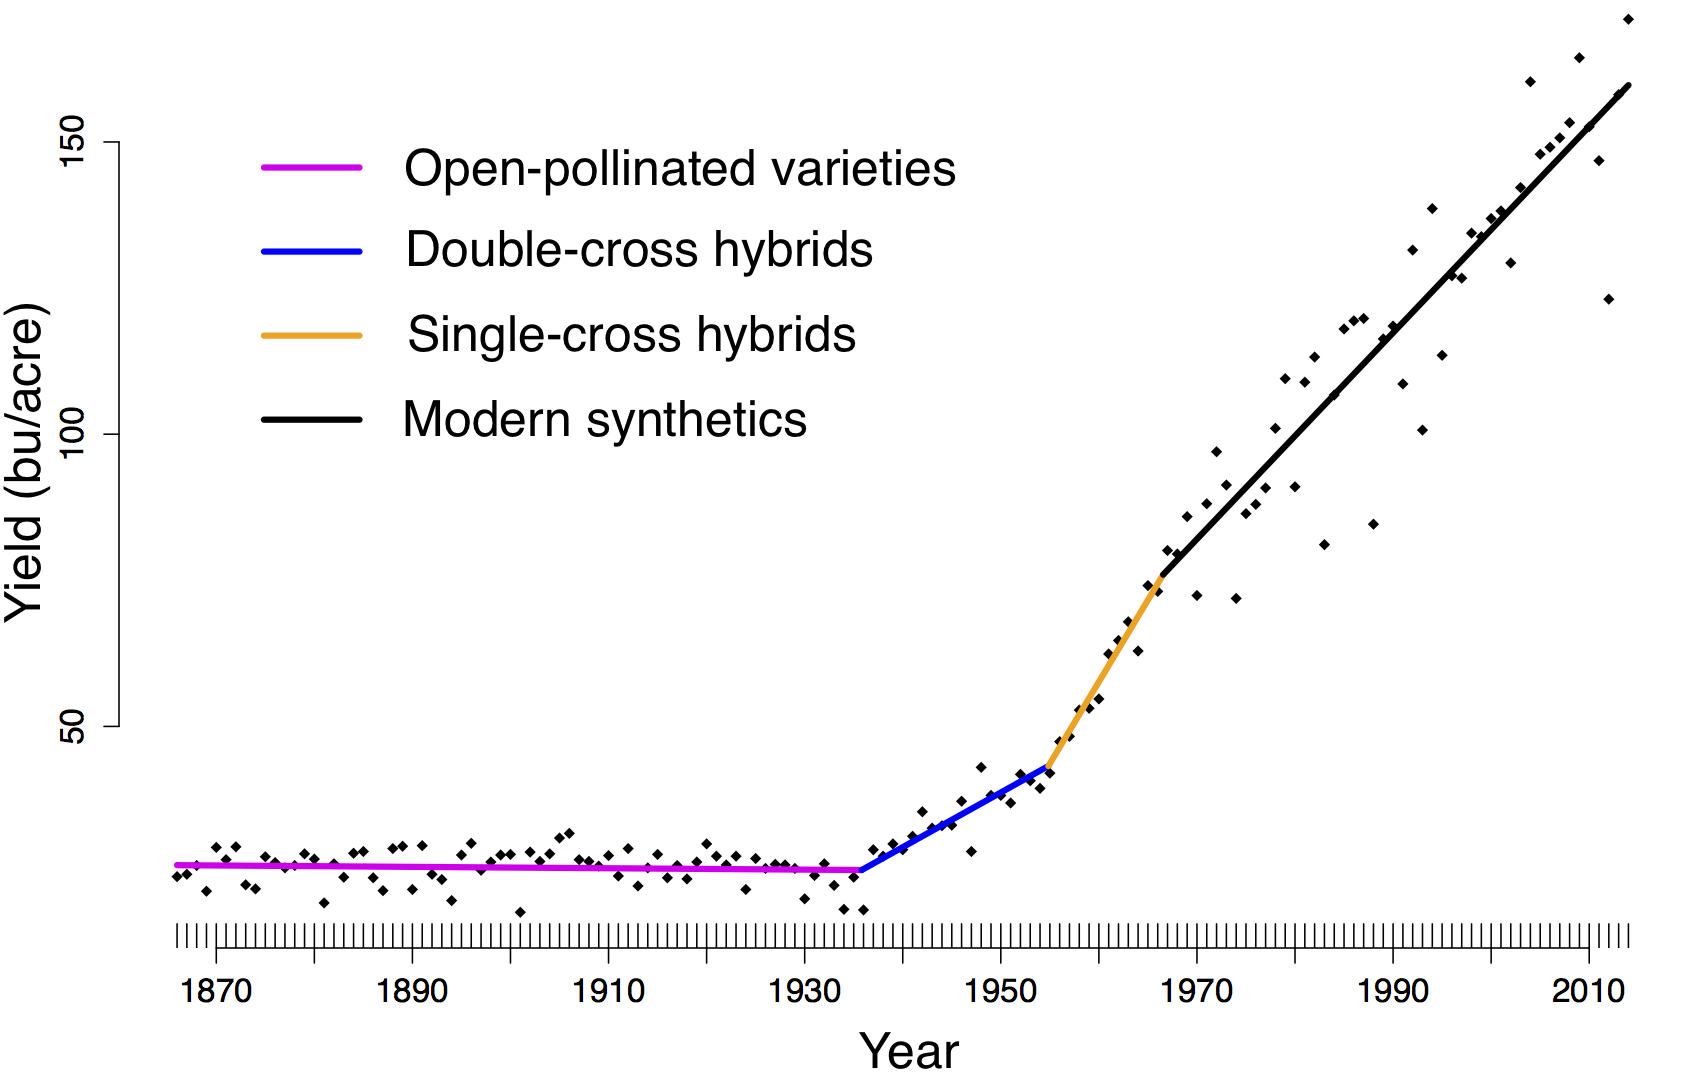
\includegraphics[width=0.7\linewidth]{yield.png}
\caption{Piecewise regressions of time against total yield through the four eras of modern maize breeding. Colors represent distinct eras of maize breeding that roughly correspond to the eras  referred to in Figure \ref{fig:diversity}.} 
\label{fig:piecewise}
\end{figure}

As selection progresses within a breeding program, inbred lines with poor performance are generally discarded, leading to a decreased effective population size ($N_e$) of the breeding pools.
Response to selection is proportional to the additive genetic variance $V_A$ (equation \ref{eq:lush}), and $V_A$, in turn, depends on $N_e$ as well as the mutational variance per generation ${\sigma}_m^2$ \citep{whitlock1999neutral}:

\begin{align}
E[V_a] = 4N_e {\sigma}_m^2
\label{eq:whitlock}
\end{align}

A reduction in $N_e$ thus inherently leads to a reduced response to selection, leading to diminishing returns on yield unless new diversity is brought back into breeding pools.
Evidence from the Iowa Reciprocal Recurrent Selection breeding program suggests these concerns are valid (Figure \ref{fig:trends}), as yield gains plateau over time \citep{rouse2003selection} concomitant with continued declines in genetic diversity \citep{Gerke:2013tw}.
Decreasing $N_e$ (Figure \ref{fig:diversity}) in U.S.  germplasm risks our ability to maintain or increase rates of genetic gain in yield.

\begin{SCfigure}
    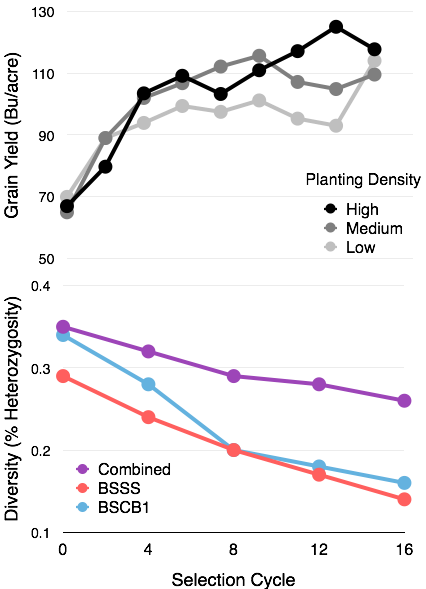
\includegraphics[width=0.45\textwidth]{BSSS.png}
  \caption{Yield and genetic diversity in the Iowa Recriprocal Recurrent Selection Program across 16 cycles of selection. (Top) Grain yield at three planting densities; data are from \citet{rouse2003selection}. (Bottom) Genetic diversity of the BSSS and BSCB1 breeding pools separately and combined; data are from \citet{Gerke:2013tw}.}
\label{fig:trends}
\end{SCfigure}

\subsubsection*{Useful diversity in old lines}
As any breeder will attest, old lines have fallen out of use precisely because they showed inferior agronomic performance under a particular selective regime (usually combining ability).
There are a number of reasons, however, why older lines may retain useful genetic diversity.
Lines are often discarded or selected against because of poor performance for a particular trait, but this does not preclude that line's utility in breeding for other traits.
Because of this, beneficial alleles for many traits of interest may remain in older germplasm, not having been advanced during breeding (Figure \ref{fig:div}).
For example, thanks to its combining ability, the U.S. inbred B73 quickly spread in popularity and now makes up a considerable portion of modern breeding material \citep{van2012historical}. 
Yet when evaluated for drought and heat stress, B73 significantly underperformed compared to less well-utilized lines such as B76 \citep{chen2012characterization}.
Analysis of a suite of diseases also finds that many less well-utilized public inbreds show greater resistance than popular lines \citep{wisser2011multivariate}. 

Most breeding programs consist of relatively small population sizes, and in these cases genetic drift can substantially impact the fate of even beneficial alleles \citep[e.g.][]{Gerke:2013tw}.
The contribution of older lines to modern germplasm thus does not necessarily reflect their genetic potential: our population genetic analysis of maize ancestry, for example, found lines with more beneficial (as defined by a steady increase in allele frequency over time) alleles than expected given their contribution to modern germplasm (Figure \ref{fig:wf9}).

\subsection*{A novel pedigree-based approach to incorporate new diversity}

Incorporating novel diversity into contemporary modern maize lines is clearly an important goal necessary to maintain or accelerate breeding and rates of yield gain.
While there are other public efforts that aim to achieve this goal, like the GEM  (Germplasm Enhancement of Maize) program \citep{pollak2003history}, these  focus on incorporating exotic germplasm (e.g. CIMMYT lines, tropical hybrids, etc.) into U.S. materials by backcrossing to well-adapted U.S. cornbelt backgrounds.
This complementary approach is good source of bringing in new diversity, but requires time-consuming back-crossing before it can generate lines that are of sufficient quality to incorporate into a breeding program.

\textbf{We propose a different approach, using pedigree data to identify underutilized cornbelt germplasm.}  
While this approach shares with projects like GEM the disadvantage that diverse material is often  agronomically inferior, it has a number of advantages.  
First, in contrast to exotic germplasm, older U.S. germplasm is already reasonably well-adapted to the daylength and climate of the U.S. \citep{Teixeira:2014hr}, meaning it can be immediately incorporated into breeding programs without first requiring extensive back-crossing.
Second, with sufficient information (see below), breeders may be able to learn a substantial amount about the potential utility of a line by predicting phenotype directly or understanding its relationship to known material. 
Finally, considerable information is available about many old breeding lines even without prediction (Figure \ref{fig:words})

\begin{figure}[t]
        \begin{subfigure}[b]{0.5\textwidth}
                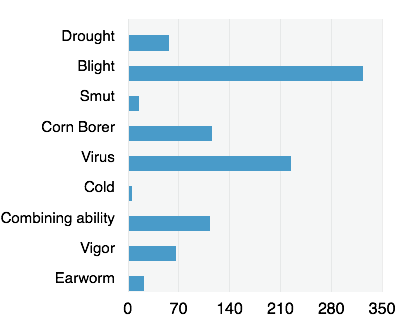
\includegraphics[width=\textwidth]{disease.png}
                \caption{}
                \label{fig:words}
        \end{subfigure}%
        ~ %add desired spacing between images, e. g. ~, \quad, \qquad, \hfill etc.
          %(or a blank line to force the subfigure onto a new line)
        \begin{subfigure}[b]{0.5\textwidth}
                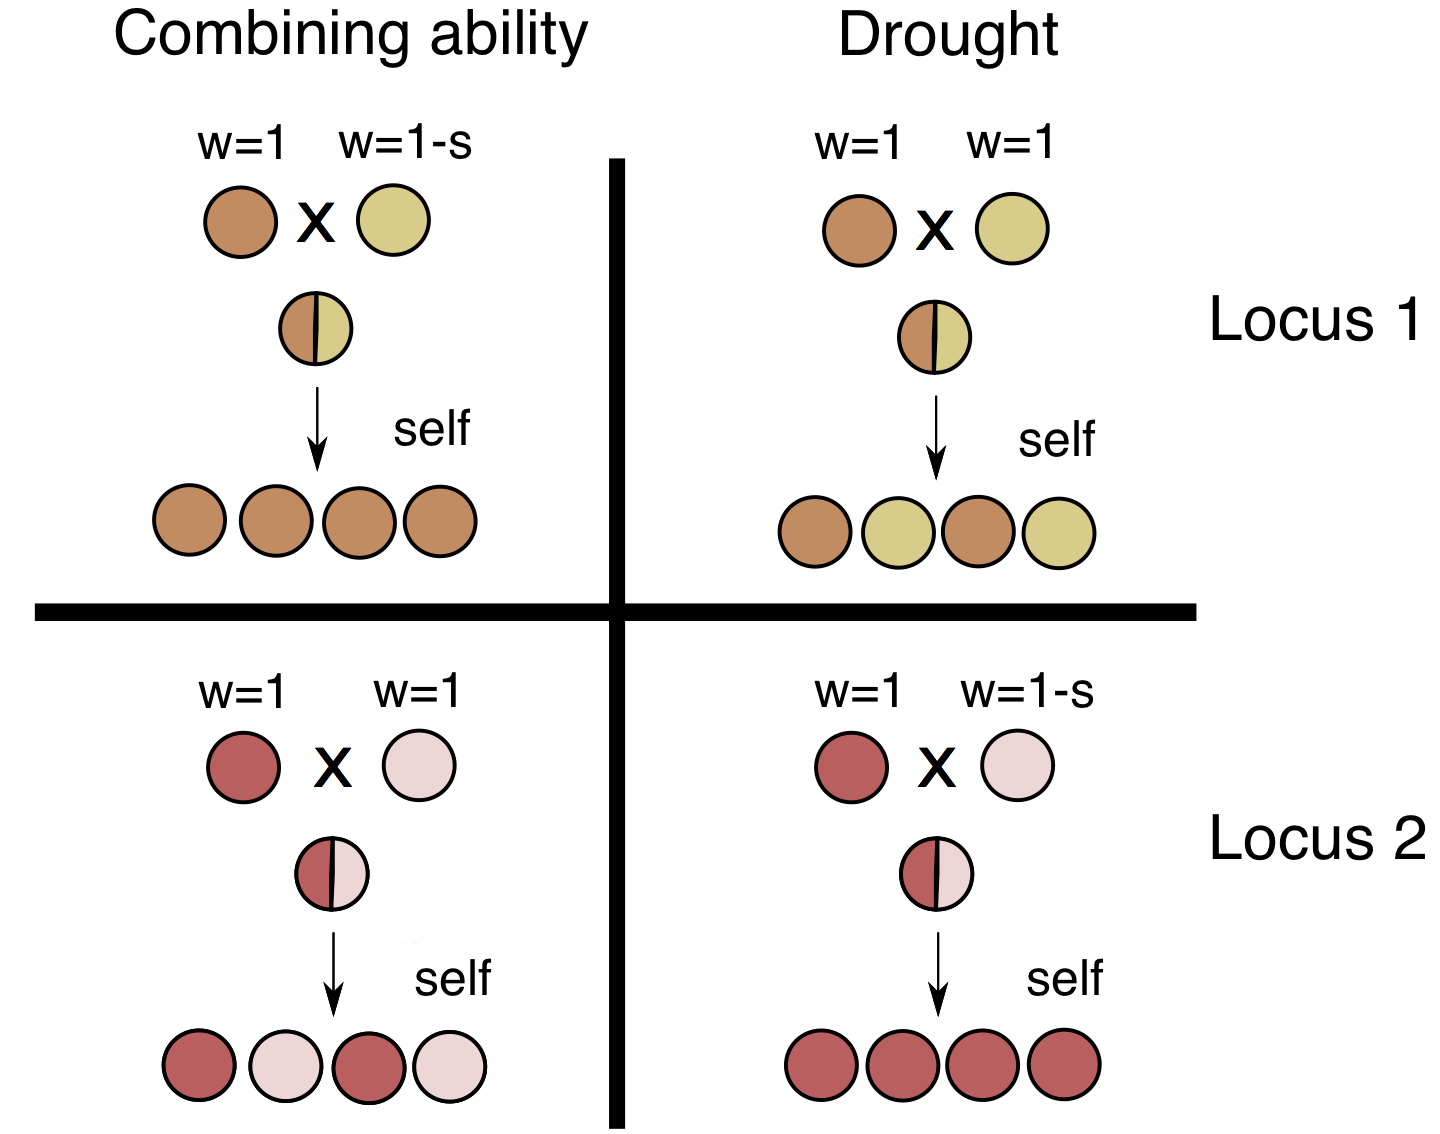
\includegraphics[width=\textwidth]{divergent.png}
                \caption{}
                \label{fig:div}
        \end{subfigure}

\caption{a) Counts of a small set of germplasm descriptors from the USDA database for which we currently have genomic and ancestral data. b) Expected segregation of alleles at loci for two traits in different breeding programs.  Selective regime for combining ability across two example breeding programs and loci. Fitness (w) of each allele indicated, with selection coefficient (1-\textit{s}) for the allele being selected against in a given regime. In each breeding program one of the alleles is effectively neutral such that older lines may still harbor useful diversity for traits which were not under selection.}

\end{figure}
 
\subsubsection*{Advantages of pedigree approaches}

Pedigree-based analysis offers a number of advantages for identifying useful diversity in older germplasm.
First, most pedigree data contain not only parentage information, but a wealth of important phenotypic data and information about the breeding program inbreds were utilized in (e.g. Figure \ref{fig:words}). 
Pedigree approaches also allow the identification of beneficial allelic diversity (e.g. Figure \ref{fig:div}, see Aim 2).
While population genetic approaches can achieve this latter goal to some extent \citep[e.g.][]{van2012historical}, they have so far failed to identify many large-effect loci, though patterns of diversity within individual breeding programs suggest such loci are likely to exist \citep{Gerke:2013tw}.
Pedigree approaches can identify strong selection within individual breeding programs (see Aim 2) without needing to average across many different programs.  
Pedigree approaches can also naturally deal with population structure, because expected relatedness is built into the pedigree itself.
Finally, pedigrees allow prediction of phenotype even in the absence of genotype \citep{piepho2008blup}.  
While this is never a substitute for growing lines in the relevant environment for comparative purposes (see Aim 3), it does save considerable time and expense and provides breeders an initial estimate of which germplasm could be most useful.

\subsubsection*{The missing data challenge}

Unfortunately, much of the pedigree information on older founder inbred maize lines sits in old volumes of Crop Science or the Agronomy Journal, experimental station technical bulletins, regional corn breeding meeting records, release sheets, or breeding books --- unaviable and vulnerable to loss.  
The National Plant Germplasm Service (NPGS) database records ancestry information, but at least 92\% of the accessions in the database have zero ancestry data, and of the 8\% that do have some ancestry data 20\% is incomplete or uses pedigree notation that is not standard. 
While private companies likely have their own pedigree databases, these data are private, patented, and not available to the public. 
\textbf{We will gather pedigree data from public sources (minutes of breeding committees, breeding program books, and other hard-copy-only sources) in order to preserve this historical information and combine it with genotyping data to accelerate future public and private (see letter of support from Dupont Pioneer) maize breeding programs.}

\subsection*{Preliminary work}
To date, we (senior personnel Drs. Oscar Smith and Kate Crosby) have gathered parentage info for over 3193 lines from a variety of sources, including \cite{gerdes1993compilation}, the NPGS, patent variety protection records, inbred release publications, and communication with breeders.
We have standardized names across these datasets and stored these data in a SQL database, which can be queried by common name (e.g. ``B73'') as well as unique NPGS identifiers (``PI 550473'' for B73).
We have combined these data with genome-wide genotyping-by-sequencing (GBS) data \citep{romay2013comprehensive}, and built a large pedigree of $\approx$700 lines (Figure \ref{fig:combo}a) with complete parentage and genotype information. GBS data allows us to validate recorded pedigrees, identifying parental combinations that are impossible given the genotyping data (Figure \ref{fig:combo}b).

\begin{figure}
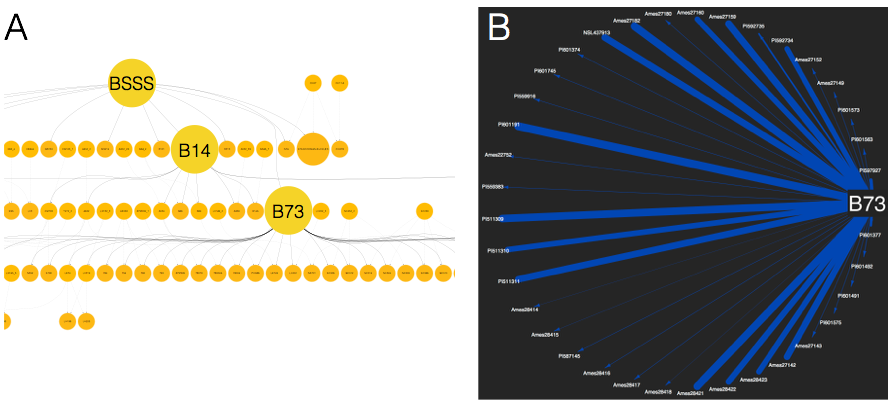
\includegraphics[width=1\linewidth]{crosby_combo}
\caption{A) A small portion of our current pedigree, showing partial data for inbred  B73. B) Pedigree of putative first-generation descendants of inbred B73. Blue arrows are weighted by the relatedness estimated from identy-by-state using GBS, clearly showing multiple errors in the putative pedigree.}
\label{fig:combo}
\end{figure}

\section*{Approach}
\label{sec:approach}
Our proposed research has three major aims in identifying and utilizing diversity to accelerate maize breeding.

\begin{itemize}
\item Aim 1: Digitize and curate pedigree and genotype information into a publicly available database. 
\item Aim 2: Identify useful diversity using a combination of pedigree and population genetic approaches.
\item Aim 3: Field test individuals lines that feature heavily in the historical pedigree.
\end{itemize}

\subsection*{Aim 1: Public pedigree curation}
Our first aim is stop the potential loss of hard copy pedigree data by gathering it from land grant institutions that previously hosted breeding research programs of maize inbred lines. 
Land grant schools of primary importance were identified by Co-PI Dr. William Tracy and  Dr. Smith (senior personnel), who have between them have more than 70 years of breeding experience in maize. 
Dr. Tracy was senior author on the leading pedigree book of maize lines \cite{gerdes1993compilation} and Dr. Smith spent 7 years working as maize breeder for the USDA (including working on the Iowa RRS population), follow by more than 20 years as a maize geneticist for Dupont Pioneer. The ``high-priority'' land grant schools they have identified include: the University of Wisconsin, Virginia Tech, the University of Georgia, the University of Florida, Pennsylvania State University, the University of Nebraska, North Carolina State University, and the USDA station at the University of Missouri. 

Co-PI Tracy and Co-PI Holland's student will largely be responsible for visiting these schools in the first year to obtain and digitally scan this information with portable digital scanners. 
Co-PI Wisser's student will be responsible for visiting two schools starting in the second year of the grant.
Co-PI  Tracy will obtain information from the University of Wisconsin (host institution), the University of Florida, and the University of Nebraska. 
Co-PI Holland's student (in the first year) will be responsible for North Carolina State University (host institution), the University of Georgia.
Dr. Sherry Flint-Garcia (senior personnel) has agreed to obtain and pass along records from the USDA station at the University of Missouri. 
Co-PI Wisser's student (to start in year two of the grant) will be responsible for the University of Pennsylvania and Virginia Tech.
Drs. Tracy and Smith have extensive contacts with faculty past and present at these schools, so obtaining the information and scanning it at each school traveled to should take no more than a few days. 

Optical character recognition software will be used where possible to automate extraction of information from scans, but we imagine a fair amount of hand-curation will be required.
Dr. Crosby (senior personnel), Dr. Taner Sen (support letter from maize GDB enclosed), senior personnel Dr.  Smith, and Co-PI Dr. Tracy will consult on an agreed upon standard format for recording data from scans.
Standardized formatting will enable consistent mapping of current and future genomic data formats to pedigree information. Both the raw scans of pedigree records and our data sheets which will be made available publicly with permanent, unique doi (digital object identifier) via services such as Github (\url{www.github.com}) or Figshare (\url{www.figshare.com}).
We will translate current and new phenotypic data into standardized maize ontologies such as those supported by the Generation Challenge Program \citep[\url{http://www.cropontology.org/ontology/CO_322/Maize}, ][]{shrestha2012bridging}

We anticipate that we will identify some lines that feature heavily in the historical pedigree but that do not have any genotypic data available for them. 
To facilitate downstream applications (see Aims 2 and 3), we will use genotype-by-sequencing (GBS) \citep{Elshire:2011ha} to obtain genome-wide genotype data.
Germplasm will be requested from the relevant sources, and germination and DNA extraction will be performed at UC Davis.  
Genotyping will be outsourced to the Genomic Diversity Facility at Cornell University (\small{\url{www.biotech.cornell.edu/brc/genomic-diversity-facility}}), and sequence data processed following standard pipelines \citep{Glaubitz:2014eu}.
We anticipate that no more than a few hundred inbred lines (2-4, 96-well plates) would need to be genotyped.

Dr. Crosby will be responsible for database generation and curation.
The initial database will continue to be in SQL format, with entries for release dates, historical phenotype information, breeder notes, germplasm availability (or nearest neighbor germplasm availability), and GBS genotype.  
While other genotyping has been performed on a number of lines, GBS is the \emph{de facto} standard \citep{romay2013comprehensive} and merging data across platforms is beyond the scope of the work proposed here. 
GBS data will be stored in hdf5 format and made available via iPlant (\url{www.http://iplantcollaborative.org}).
We will develop software to extract genotype data from specific genomic regions in subsets of lines and estimate allele sharing via identity by state (IBS) between sets of lines in specified genomic regions.
Finally, we will implement simple phenotypic prediction (see Aim 2) functionality allowing users to estimate phenotypic values based on a set of loci from genome-wide association studies.

Starting in year two of the grant, the pedigree database will be made available publicly via MaizeGDB (\url{www.maizegdb.org}), the USDA-funded central resources for maize genomics (see letter of support from Dr. Taner Sen).
We will update the database as new information arises, and provide functionality such that users can submit database updates (in the appropriate format) to MaizeGDB to ensure continued utility and availability of this resource.

\subsubsection*{Expected outcomes (Aim 1)}
Our main deliverable from Aim 1 is an \textbf{open public pedigree database to be hosted on MaizeGDB (http://www.maizegdb.org/) for the long term future.} 
In addition to providing information on pedigree, this database will house both genotype and substantial phenotype information, a combination of critical importance for continued plant breeding efforts \citep{zamir2013have}.
Users will be able to contribute and revise incomplete information, with the goal of establishing a nearly complete public pedigree of maize inbred lines.   

Example usage might include a breeder querying the database for lines with descriptors suggesting drought and blight resistance, identifying the genotype of such lines at loci thought to be associated these traits from GWAS or other studies, and use the database to predict phenotype for related material with no descriptive data.

Ensuring data, code, and script are open-access or open-source (freely available to the public) is important for critique, debate, and dialogue in science. 
Drs. Ross-Ibarra and Crosby have a long track record of ensuring openness in science, data, and code. Throughout this project, both Dr. Ross-Ibarra and Dr. Crosby will endeavor to ensure that code and data are available via permanent, publicly accessible repositories such as github, figshare, maizeGDB, and iPlant.

\subsubsection*{Potential pitfalls \& limitations (Aim 1)}

While we are optimistic about the prospect of obtaining accurate pedigree information from these various institutions, we recognize that many records will be incomplete. 
In practice, while knowing the exact number of meioses between lines would be desirable, we expect we will recover only parentage information from a large number of lines. 
Parentage alone is sufficient for allele-dropping and prediction (see Aim 2), but not knowing the number of meioses makes it difficult to know the uncertainty associated with prediction or use pedigree data to understand recombination.
 
A second challenge is that while pedigree records and other information on old lines may be available, the germplasm from these old lines may no longer be available. 
Approximately 12.9\% of germplasm from NPGS for which we have parentage information is no longer available, and we expect similar or higher levels from less accessible sources. 
We note, however, that such lines remain useful in connecting available lines together in the pedigree, and pedigree alone can be used to predict phenotype. 
If we identify historically important germplasm that is no longer available, we will identify and genotype the nearest relatives for which seed are available. 

\subsection*{Aim 2: Identify useful diversity}

In this aim we propose to use two distinct statistical genetic methods to identify potentially useful diversity from our pedigree database.  
First, we will use ``allele-dropping'' approaches to find individual loci that have been under selection.
Second, we will use quantitative genetic methods to do test for selection on individual phenotypes of interest.

\subsubsection*{Mendelian segregation on a pedigree}

The idea behind this method is simple: Mendelian genetics provides the simple null model for inheritance of alleles in the absence of selection.
As seen in Figure \ref{fig:div}, alleles under selection will show distorted patterns of inheritance.
Given pedigree information on a set of lines (Aim 1), we can use genotype data to test for selection on any locus simply by calculating the probability of the observed inheritance pattern along the pedigree given normal Mendelian segregation.
Loci that show low probabilities are likely to have been under selection.
Because this method uses the pedigree structure directly, it avoids difficulties of population structure inherent in population genetic or genome-wide association methods \citex.
This method has already been employed by industry to identify useful alleles in their own pedigrees \citep{sebastian1995method}.

One of the major advantages of this 	``allele-dropping'' approach is the opportunity it provides to test for loci under selection in a number of different contexts.
For example, because  different breeding programs selected for different traits (and this information is often available in pedigree records, e.g. Figure \ref{fig:words}), we can test for selection in a subset of pedigrees related by trait.
This allows us to identify alleles selected for drought in programs breeding for drought and alleles selected for disease resistance in programs focusing on specific diseases.
Alternatively, we can categorize breeding programs geographically, and ask whether certain alleles were selected in particular maturity zones, temperatures, or precipitation levels.
Finally, we might expect some loci to be consistently under selection in most programs -- especially those that are associated with combining ability or other widely-valued agronomic traits. 

By applying this segregation test to a number of smaller breeding programs, we will  isolate strong signals of breeder selection for an array of traits and environments. 
Identification of beneficial alleles in these pedigrees then lets us search across our entire dataset for cases in which the beneficial allele may have undergone relaxed selection in programs selecting for different traits (Figure \ref{fig:div}).
This allows us to identify useful alleles in specific breeding programs, or search for individual lines that stack useful alleles for multiple traits. 

%\begin{SCfigure}
%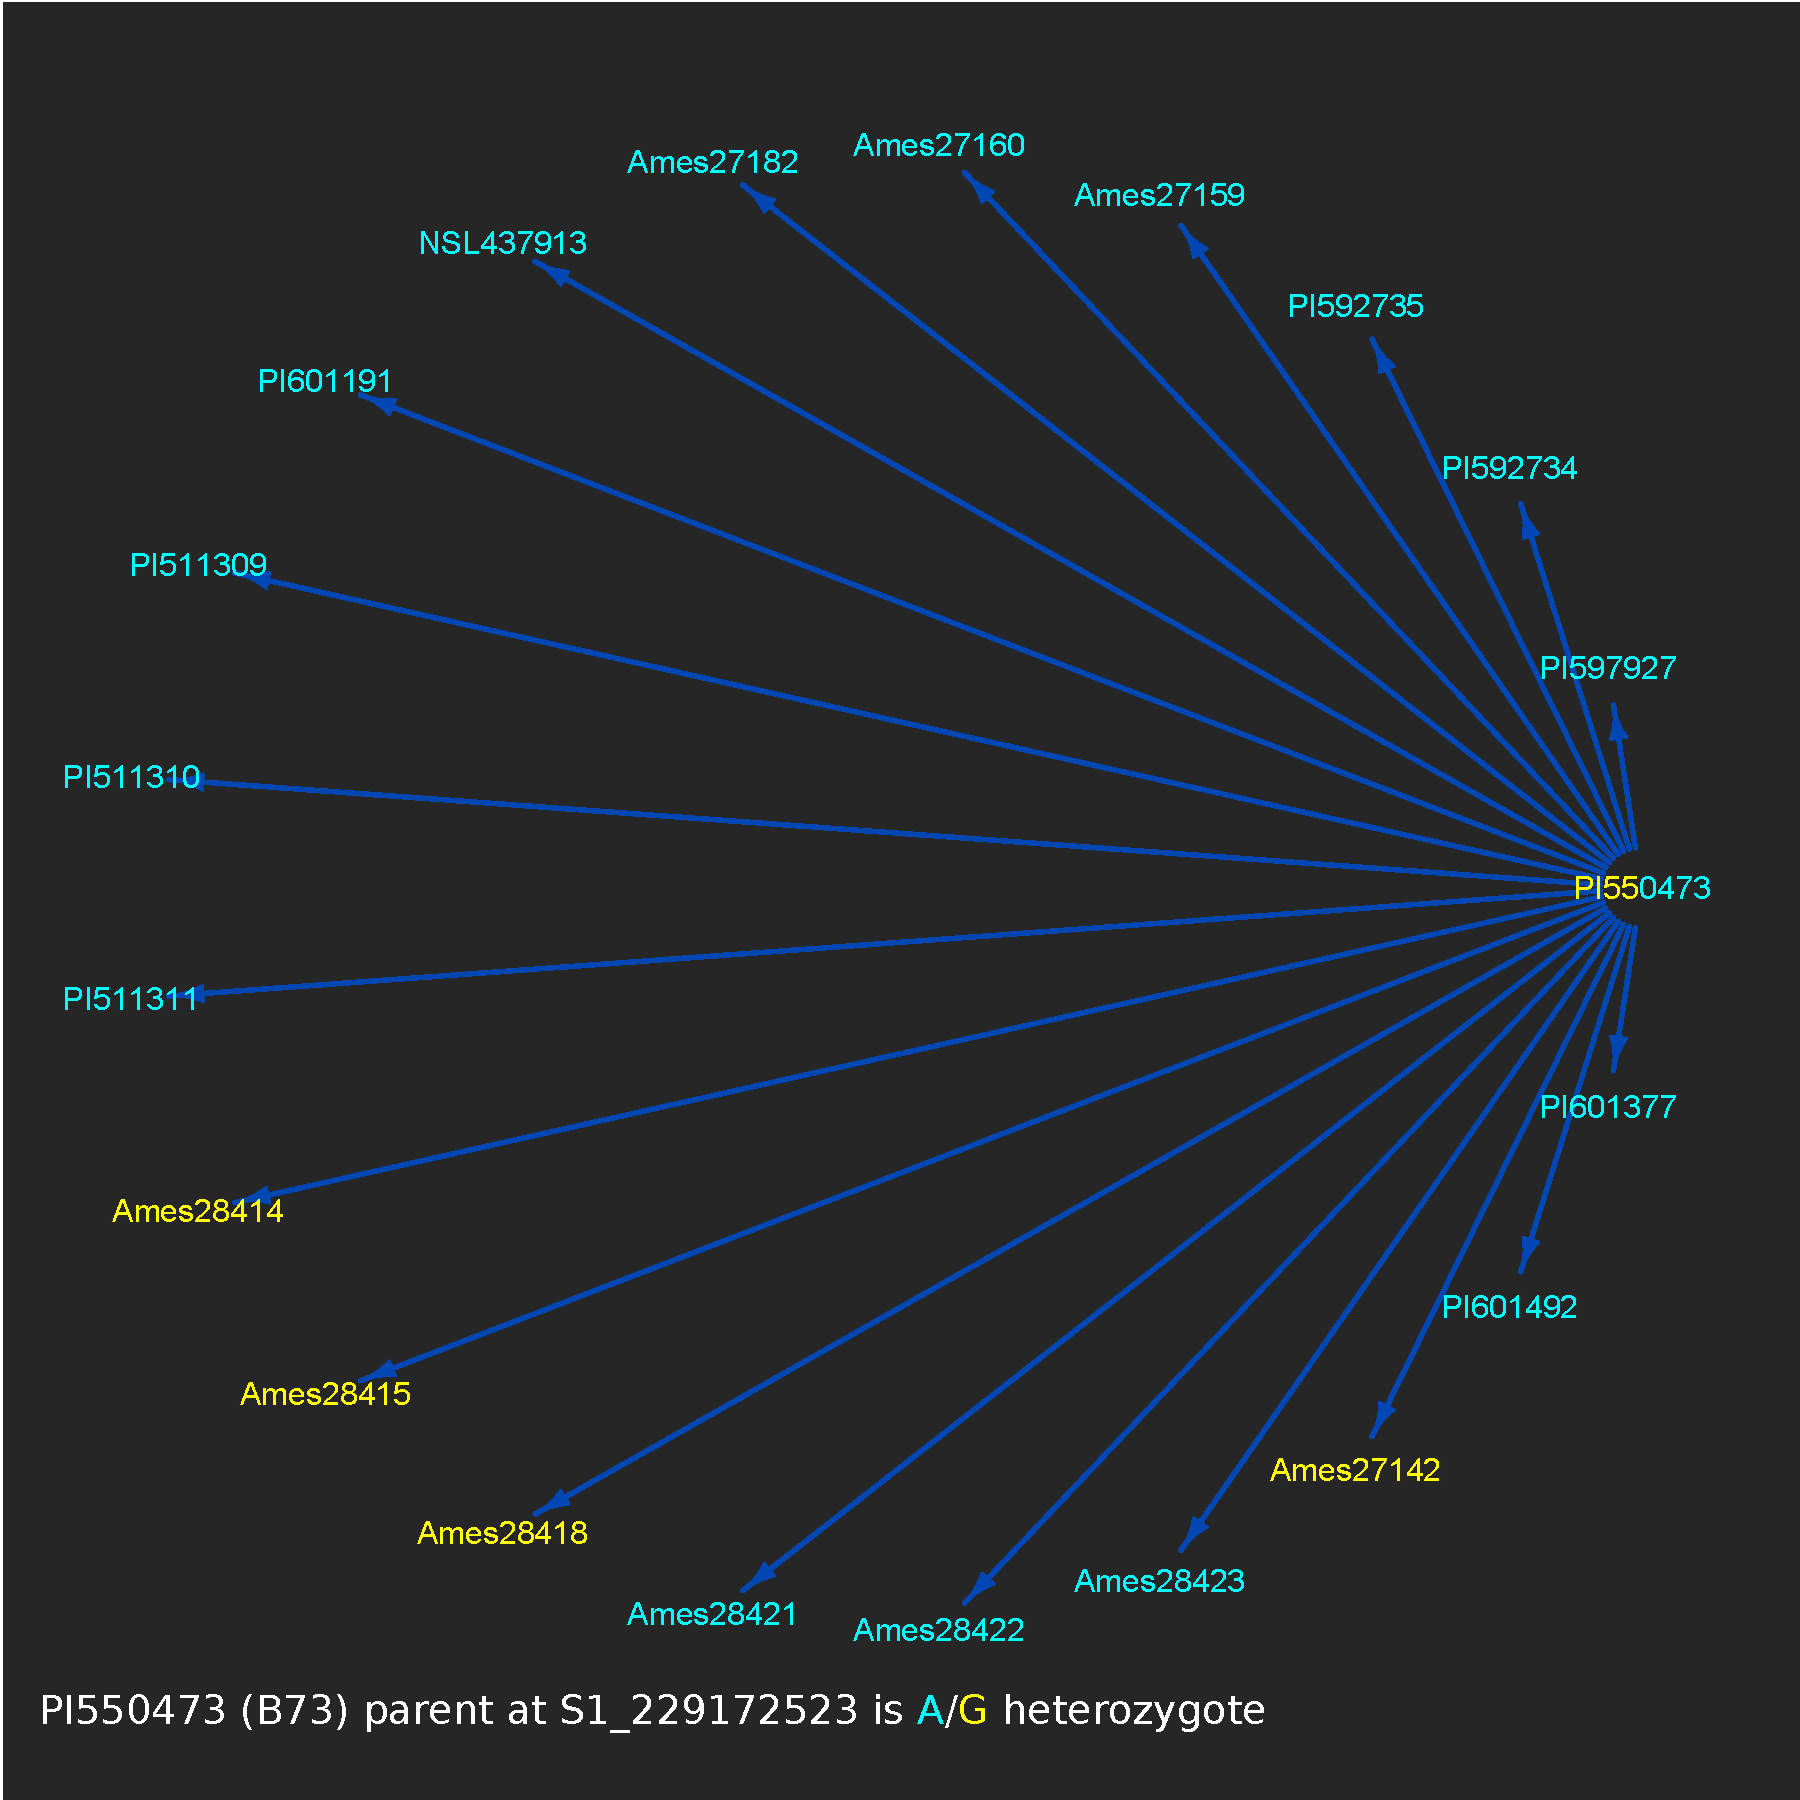
\includegraphics[width=0.5\linewidth]{Pruned.pdf}
%\caption{Inbre B73 is heterozygous at 379 loci out of over 954,000 loci with GBS markers). The blue labels represent which of its inbred progeny obtained the A allele, whereas the yellow labels indicate the progeny that have obtained the G allele at a particular locus. \textbf{NB: the other parent of these lines is not indicated for simplicity}.}
%\label{fig:alleledrop}
%\end{SCfigure}

\subsubsection*{Phenotypic selection (Aim 2)}

In the above ``allele-dropping'' approach we seek to identify individual alleles of interest.
Here, we complement those methods by identifying phenotypes that show evidence of selection.
Many crop phenotypes are highly quantitative, and in such cases population genetic or segregation tests may not have high power to detect selection on any of the many individual loci each under weak selection.
Recently developed quantitative genetic methods, however, circumvent this problem by asking whether groups of SNPs identified \emph{a priori} from GWAS analysis show concerted changes in linkage disequilibrium and frequency \citep{Berg:2014bs}.
For a given population (or individual) the method estimates the genetic value $Z$ of a trait by summing over the estimated effect sizes $\alpha$ of the $L$ GWAS hits weighted by their frequency $p$ (for diploid individuals the frequency would be 0,0.5,or 1 ): 

kc\begin{align}
    Z = \sum_{i=1}^L\alpha_ip_i
	\label{eq:berg}
\end{align}

Using genome-wide SNPs to control for population structure or relatedness, the method can then calculate the probability of the observed genetic values, with extreme probabilities suggestive of the action of selection.
We will first test this approach in breeding programs in which we know the selection applied by breeders and we have empirical data on the response.
Assuming we can find evidence of selection where we know it should be, we will then apply the method to scan across our pedigree for evidence of selection at a number of traits.

We will test for selection using data on genome-wide association results from more than 40 traits analyzed in the large nested association mapping (NAM) population \citep{wallace2014association}.  
We predict not only that we will find evidence of selection for traits that we know have been selected, but that many traits may show evidence of selection in the absence of pedigree data supporting conscious selection by the breeder.
This allows us to identify breeding populations or lines that have responded to selection for a phenotype, even if the individual loci responsible remain only partially known.

%Briefly, the approach $Q_{x}$ uses SNP hits and their allelic effects (breeding values) across the genome from a GWAS analysis. The effects sizes of these breeding values can be summarized by comparing to a random set of SNPs in that population. Here, allelic effects $\alpha^{2}$ (or breeding values), the same values that  breeders can take advantage to get an estimate of $V_{A}$ for any trait of interest. $V_{A}$ can be estimated for one locus or summarized across all loci $L$ in the genome (equation \ref{eq:berg} below):

%\begin{align}
%    V_A = 2p(1-p)\alpha^2 = \sum_{l=1}^L\alpha^2_l2p_l(1-p_l)
% % \end{equation}\break
% % \begin{equation}
% %    = \overset{L}{\underset{l=1}{\sum}}\alpha^2_l2p_l(1-p_l)
%	\label{eq:berg}
%\end{align}

%
%These hits are then projected to the expected breeding value based on the genotype of individuals in another environment (where the phenotype has not actually been observed). 

%We will test for  GWAS results from the In the case of maize, we have phenotypic data from contemporary lines from various mapping populations and their genotypes,, e.g. the large-scale Nested Association Mapping population (NAM) of thousands of recombinant inbred lines (RILs), which was developed ten years ago from 25 of the original founders of modern US germplasm \citep{mcmullen2009genetic}. 

%If alleles are at high frequency in certain breeding programs and can also associated with a beneficial phenotype (e.g. blight resistance), they are potentially beneficial alleles that could be resurrected and introgressed back into a modern breeding program. 
%By then searching the entire pedigree for these alleles and isolating those lines that have these SNPs, they may be targeted by breeders and public research programs.
%Further, the greater the $V_A$ of a trait (the greater the allelic diversity of that trait, i.e. $N_{e}$), and thus, the greater $R$ (response to selection) to any new selective program a breeder chooses to apply.

%\begin{SCfigure}
%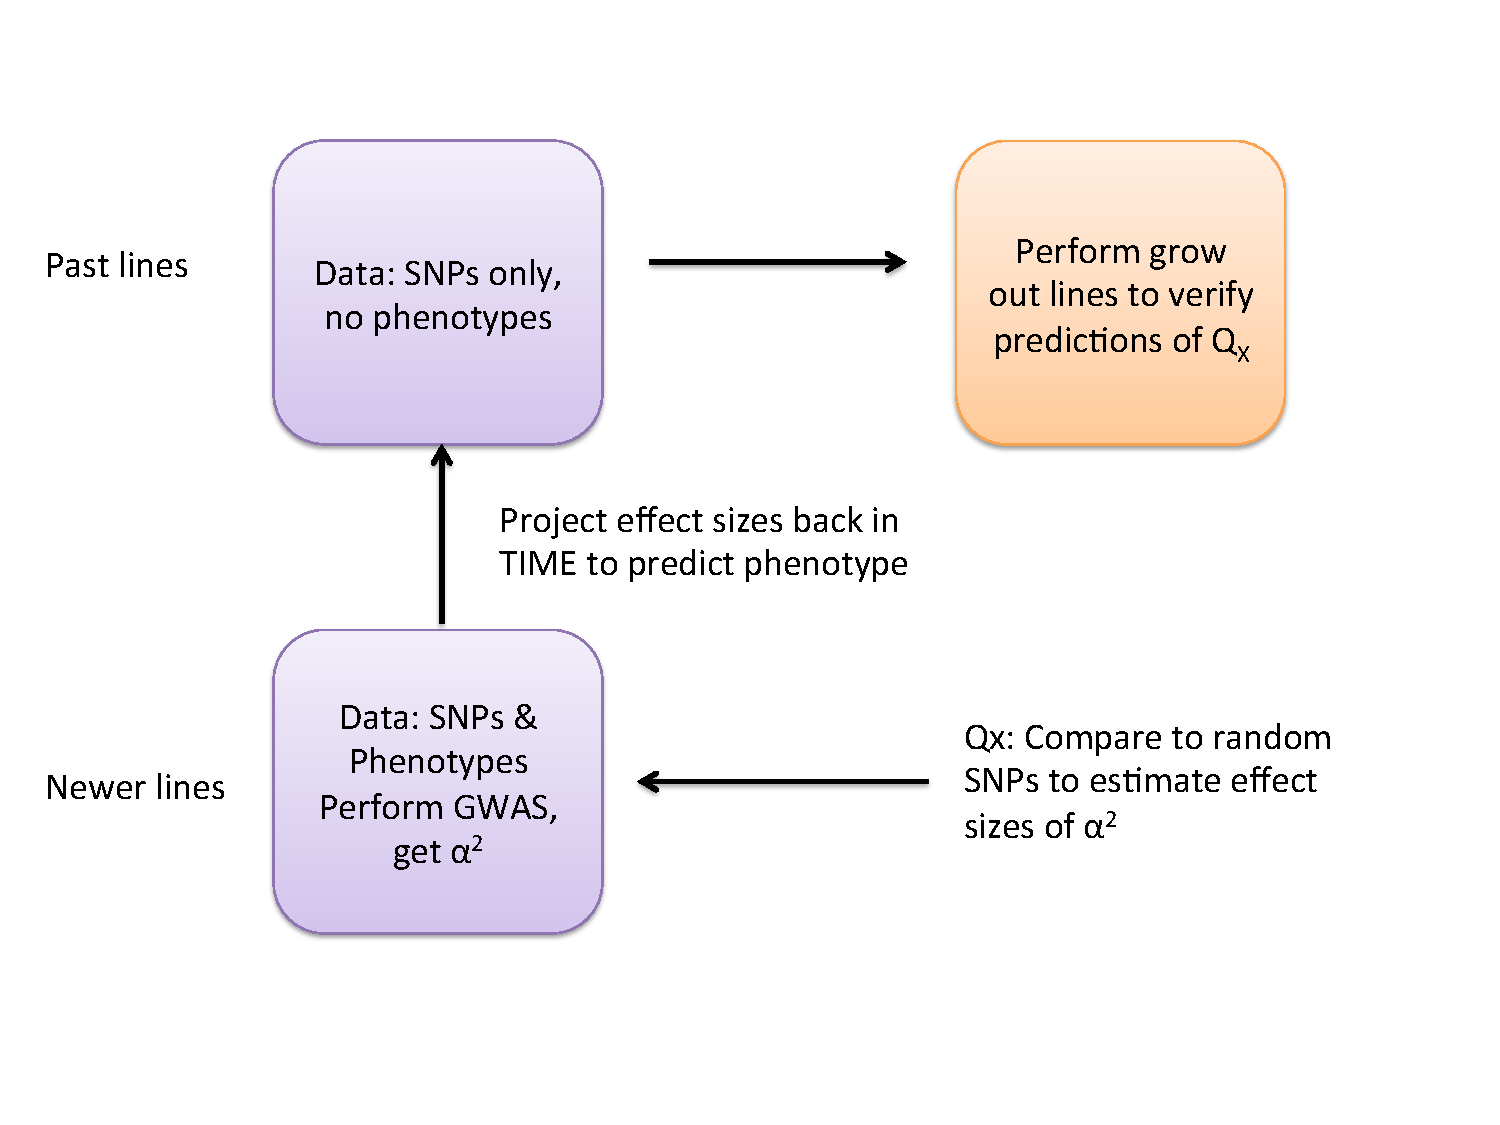
\includegraphics[width=0.7\linewidth]{Qx.pdf}
%\caption{Simple schematic of how the $Q_{x}$ approach works}
%\label{fig:qx}
%\end{SCfigure}

\subsubsection*{Expected outcomes (Aim 2)}

The idea of applying these two complementary approaches is to identify potentially useful diversity from our pedigree databse.
SNPs identified by allele-dropping can be tagged in the database for future reference, and breeding programs or lines showing evidence of selection for specific phenotypes can be noted as well.
These notations may be of use for breeders, though we expect breeders interested in subsets of the germplasm or specific traits would want to run additional analyses.
Each analysis will be run by one of the two masters students employed on the grant, providing them with statistical genetics training and an analytical skill-set desirable for applied industry or public research. 

\subsubsection*{Potential pitfalls \& limitations (Aim 2)}
%Genotypes when combined with a pedigree can be used to predict phenotypes \citep{de2009predicting,crossa2010prediction,Decker:2012kd}.
%By using allele dropping we target individual loci within and across breeding programs, associating high frequency SNPs with their given selective regime (drought, disease, etc). 
There are two potential limitations with the allele-dropping approach. First, there may be a lack of statistical power in detecting selection on individual alleles, because there may be too few progeny of each line under a given selection regime. 
Secondly, allele dropping may not have the statistical power to detect a more diffuse polygenic signal of adaptation spread across many alleles in a genome (similar the drawbacks of using traditional QTL mapping and $F_{ST}$ scans) \cite{Rockman:2011ej, Berg:2014bs}. 
Both of these limitations are circumvented to some degree by our second approach, which can look across a broader set of arbitrarily related germplasm for a large number of loci.
This second approach, however, may exhibit high false positive rates if gentic structure in the test population is correlated with that of the original GWAS panel \citep{Berg:2014bs}. 
This is an area we are actively investigating; while we have not resolved it to our satisfaction yet we suspect that by re-running the GWAS with subsets of the diverse NAM panel much of this problem can be ameliorated.  
\subsection*{Aim 3: Field testing individual lines}

Our final aim is to use small-scale grow-outs to validate our approaches in Aim 2 and test the utility of older lines as viable sources of diversity for breeding.
We will perform two grow-outs in years 2 and 3 of the grant (see timeline below).
First, we will choose a single trait (for simplicity likely a disease resistance) for which we selection was undertaken in a large number of programs in our databse.
We will perform allele-dropping (see Aim 2) for this trait, and choose the 40 lines with the lowest and 40 lines with the highest number of beneficial alleles.
These will be accompanied by a set of 40 ex-PVP inbreds representing the most elite germplasm available to the public. 
Attempts will be made to match groups based on maturity and time period (so as not to compare many 1940's lines with 1980's lines).
Here we predict that lines with more of the beneficial alleles will have more desirable phenotypes for the trait of interest.

We will choose a second trait of interest for the second experiment in year 3.  
Using the prediction approaches outlined in Aim 2, we will identify breeding programs that have not bred for the trait (or more likely for which there is no information to suggest that they have bred for the trait) but nonetheless show evidence of selection on the phenotype.  
We will then choose 40 lines from early in these programs and 40 lines from late in these programs, accompanied by the same set of 40 ex-PVPs and again matching groups based on maturity and time period as much as possible.
Here we predict that later lines in these breeding programs should show more desirable phenotypes for the trait of interest than earlier lines from the same programs.  
For each experiment, we will grow 2 plots of each inbred and 2 checks in a randomized field design at the field station in U. Delaware. 
The middle 5 plants of each plot will be phenotyped for the trait of interest as well as a set of phenotypes of general agronomic interest (standability, flowering time, plant height, ear height, leaf angle, 50k weight, and yield).

\subsubsection*{Expected outcomes: Aim 3}
This aim will achieve three goals.
First, it will allow validation of phenotypes listed in the pedigree database, to give an idea of the accuracy of our records.
Second, it will allow preliminary testing of the utility of our proposed population genetic approaches in identifying germplasm of use for traits of interest.
Finally, growouts of a diverse set of older germplasm in comparison with ex-PVPs will provide useful perspective for breeders on the relative agronomic value of older germplasm as well as how ``elite'' material compares to older material for specific traits of interest.
We predict that we will be able to show that our pedigree-based methods in Aim 2 allow us to successfully choose germplasm that out-competes elite lines for specific traits of interest. 

\subsubsection*{Potential pitfalls \& limitations (Aim 3)}
Ideally, field-testing of these lines would be more comprehensive, including more replication, better controls, and multiple environments.
Given the space and time constraints of this grant, however, we feel this design is a  reasonable compromise.

Two of the most likely pitfalls relate to limited availability of germplasm. 
If numbers of seed at germplasm repositories are insufficient, we may be unable to reach the 40 lines desired or the available lines may be very unbalanced (e.g. many new lines, a few older lines).  .   
Additionally, as we will be working with older germplasm, it is possible that some lines will fail to germinate, resulting in unequal numbers with which to test our assumptions. 

\subsection*{Research Timeline}
A graphical timeline of our three-year proposal is presented below (Figure \ref{fig:timeline}).
The first year will be spent traveling and gathering and digitizing pedigree records at land-grant institutions.
Dr. Tracy and Dr. Holland's  student will be responsible for traveling to and scanning hard-copy records into digital format.  We estimate that this should take no longer than a few days at each institution.

The scanned digital records will then be translated into a usable data format for further analysis by Dr. Crosby.  Dr. Crosby will ensure that a functional version of the database is available at Maize GDB by the end of the first year; she will act as database manager throughout the proposal to the end of the third year.

Dr. Smith will consult as needed with both students (see roles below) and Dr. Crosby throughout the grant as an expert on the naming and potential ancestry of lines.

\begin{figure}
\centering
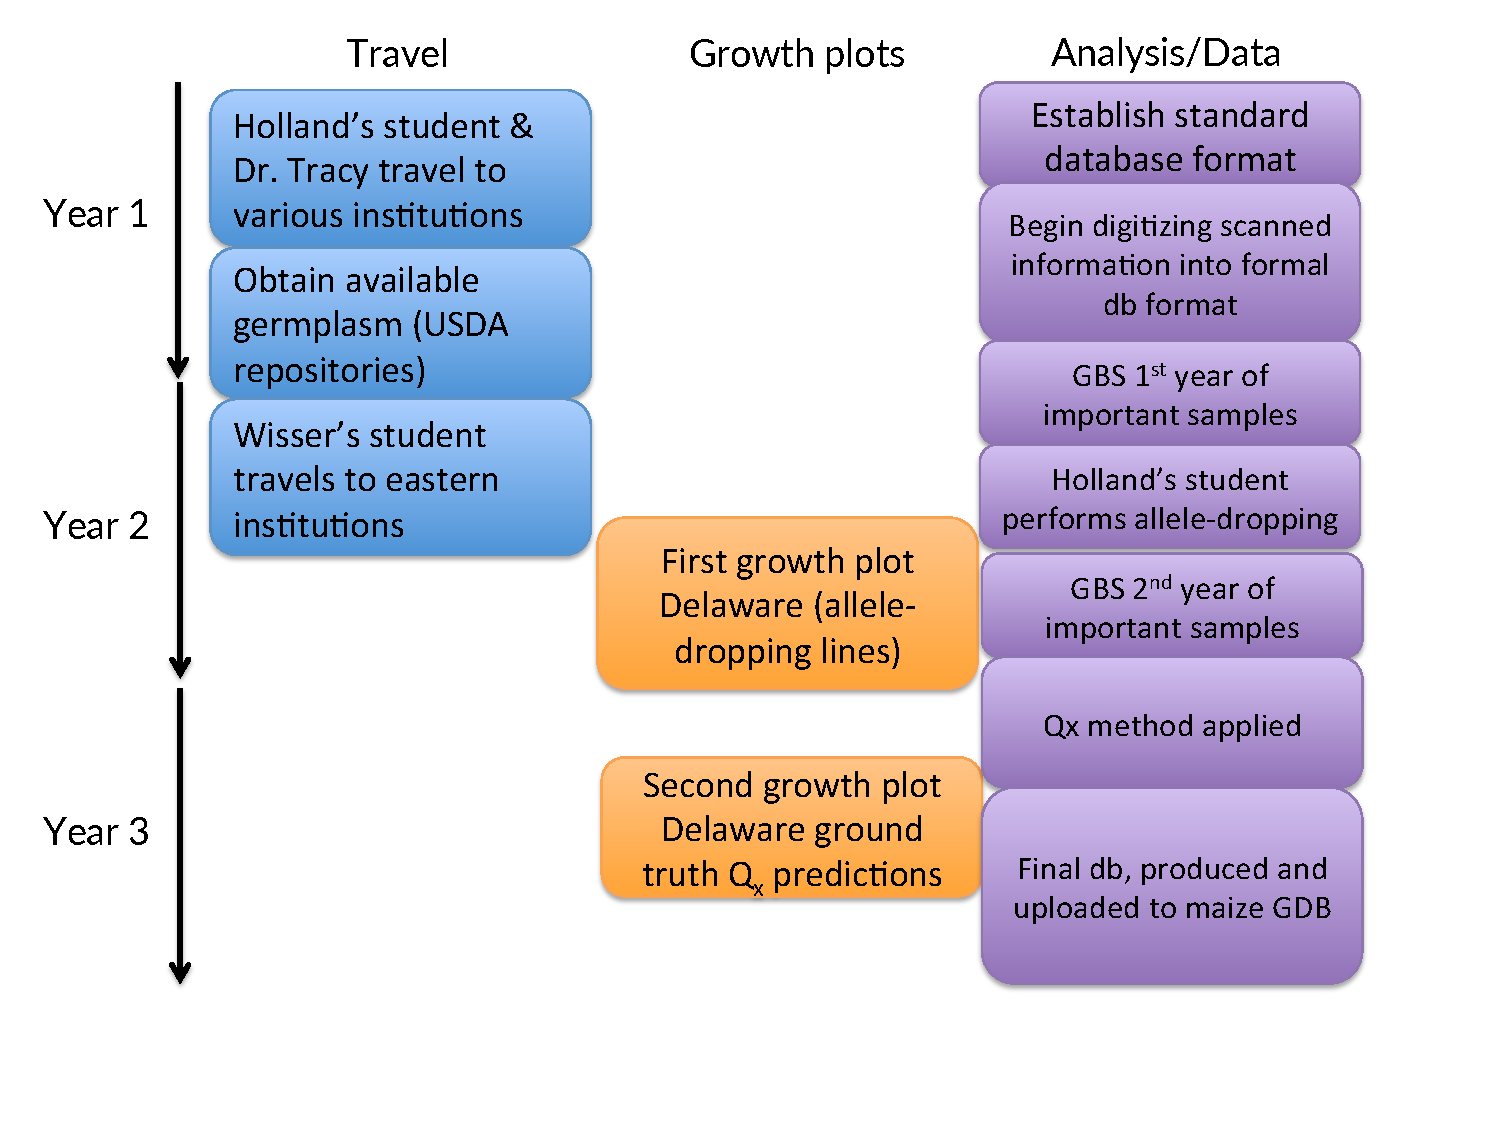
\includegraphics[width=0.7\linewidth]{timeline.pdf}
\caption{Graphical timeline of the major parts of our proposal.}
\label{fig:timeline}
\end{figure}

At the end of the first year/start of the second year, we will genotype inbred lines with available germplasm and that are well-represented in the pedigree but lack GBS data. 
Dr. Crosby will be responsible for this aspect of the project, and Dr. Holland's student will receive training in GBS analysis from Dr. Crosby. 

During year 2, Dr. Holland's student will apply allele-dropping approaches to pedigrees in the database. 
S/he will also be responsible for obtaining available germplasm of lines for phenotyping. 
In year 2, Dr. Wisser's student will visit two land grant schools in the east (Virginia Tech and the University of Pennsylvania) to obtain additional records and submit an update to the database. 
Dr. Wisser's student will also grow out the lines identified by Holland's student. 
These lines will be phenotyped by a combination of Wisser/Holland students.

In the final year (year 3), Dr. Wisser's student will apply the $Q_{x}$ method to identify phenotypes under selection and predict phenotype of under-utilized lines.
During year 3 Dr. Wisser's student will perform the second grow-out to test predictions of the $Q_{x}$ method.

Throughout the grant we will have monthly group conference calls to discuss progress, challenges, and logistics. 

As a final step, all phenotypic data, identified SNPs of related to various production traits, and ancestry information, will be transferred from Dr. Crosby's working database to maize GDB, and managed by administrators there for the long term future.

\subsection*{Broader Impacts}

\subsubsection*{Training}
Our proposal helps train two students in bioinformatics, population and quantitative genetics, plant-breeding, experimental design, statistics, and database management. 
All these applied skills that the students develop will help them in future careers, whether academic or industry. 
They will both meet and work with some of the premier experts in maize breeding (Drs. Tracy \& Smith). 
Both students will be expected and encouraged to attend the maize genetics conference, to present their results and network with working professionals from academia, government, and industry.

Both students will work alongside Dr. Crosby as well as their respective advisors to plan out analyses, troubleshoot, and advance project goals. 
Dr. Crosby, in turn, will gain valuable experience helping to mentor students along with their main advisors Drs. Wisser and Holland. 

\subsubsection*{Public Pedigree database}
Private companies such as Monsanto and Dupont Pioneer have their own pedigree databases and information that they can draw from in order to breed new hybrid commercial varieties. 
Even so, our colleagues at Dupont Pioneer (see letter of support) recognize the utility such a database would have for their breeding programs.
Public researcher and smaller breeding companies  (both in the United States and in countries abroad) often do not have the resources to develop and maintain well-curated pedigree information. 
Our proposal aims to make this information --- pedigree, phenotype, and genotype --- accessible to public breeders.
Hosting the database on maizeGDB will allow the information to be maintained and updated well beyond the timeline of this three-year project.

\subsubsection*{Application to other crop systems}
Few other crops have attempted to comprehensively take advantage of old diversity as proposed here.  
Yet, useful diversity does exist in old lines of other species \citep{gamuyao2012protein}. 

We hope that a full examination of the utility of older germplasm in one crop system (maize) may act as a stimulus for other researchers in other crops to act quickly to preserve hard-copy records and germplasm associated with these records. 
With relatively minor changes to phenotypic ontogeny and mechanisms to access different genotype data, our database could be easily ported to use in other systems as well. 

\newpage
\bibliography{kc.bib,jri.bib}
\end{document}